% Chapter for background.

\chapter{Background}
\label{ch:background}

In this chapter we discuss essential background information to this project.
First, we discuss the specific terminology used in this paper. Next, we discuss
previous work relating to this project.

\section{Technical Background}

As this project introduces a new teaching tool for 6.01,
let us first discuss the scope of circuits in 6.01.

\subsection{Circuit Components}

The rudimentary circuit components used in 6.01 are resistors, operational
amplifiers (op-amps), and potentiometers (pots). In addition to these basic
parts, students may build circuits to control LEGO motors or to control
aspects of robots designed specifically for 6.01. One of the 6.01 robots is
depicted in Figure \ref{fig:robot}. The robots can be equipped with heads that
contain three parts held together by a shaft: a LEGO motor, a potentiometer, and
a circuit card containing two photosensors. The robot in Figure \ref{fig:robot}
has a
head attached. To connect a layout to a LEGO motor, a student would use a 6-pin
connector, and to connect a layout to a robot or a robot head, a student would
use an 8-pin connector. Figure \ref{fig:components} displays all of the circuit
pieces a 6.01 student may use to build a protoboard layout.

\begin{figure}
\begin{center}
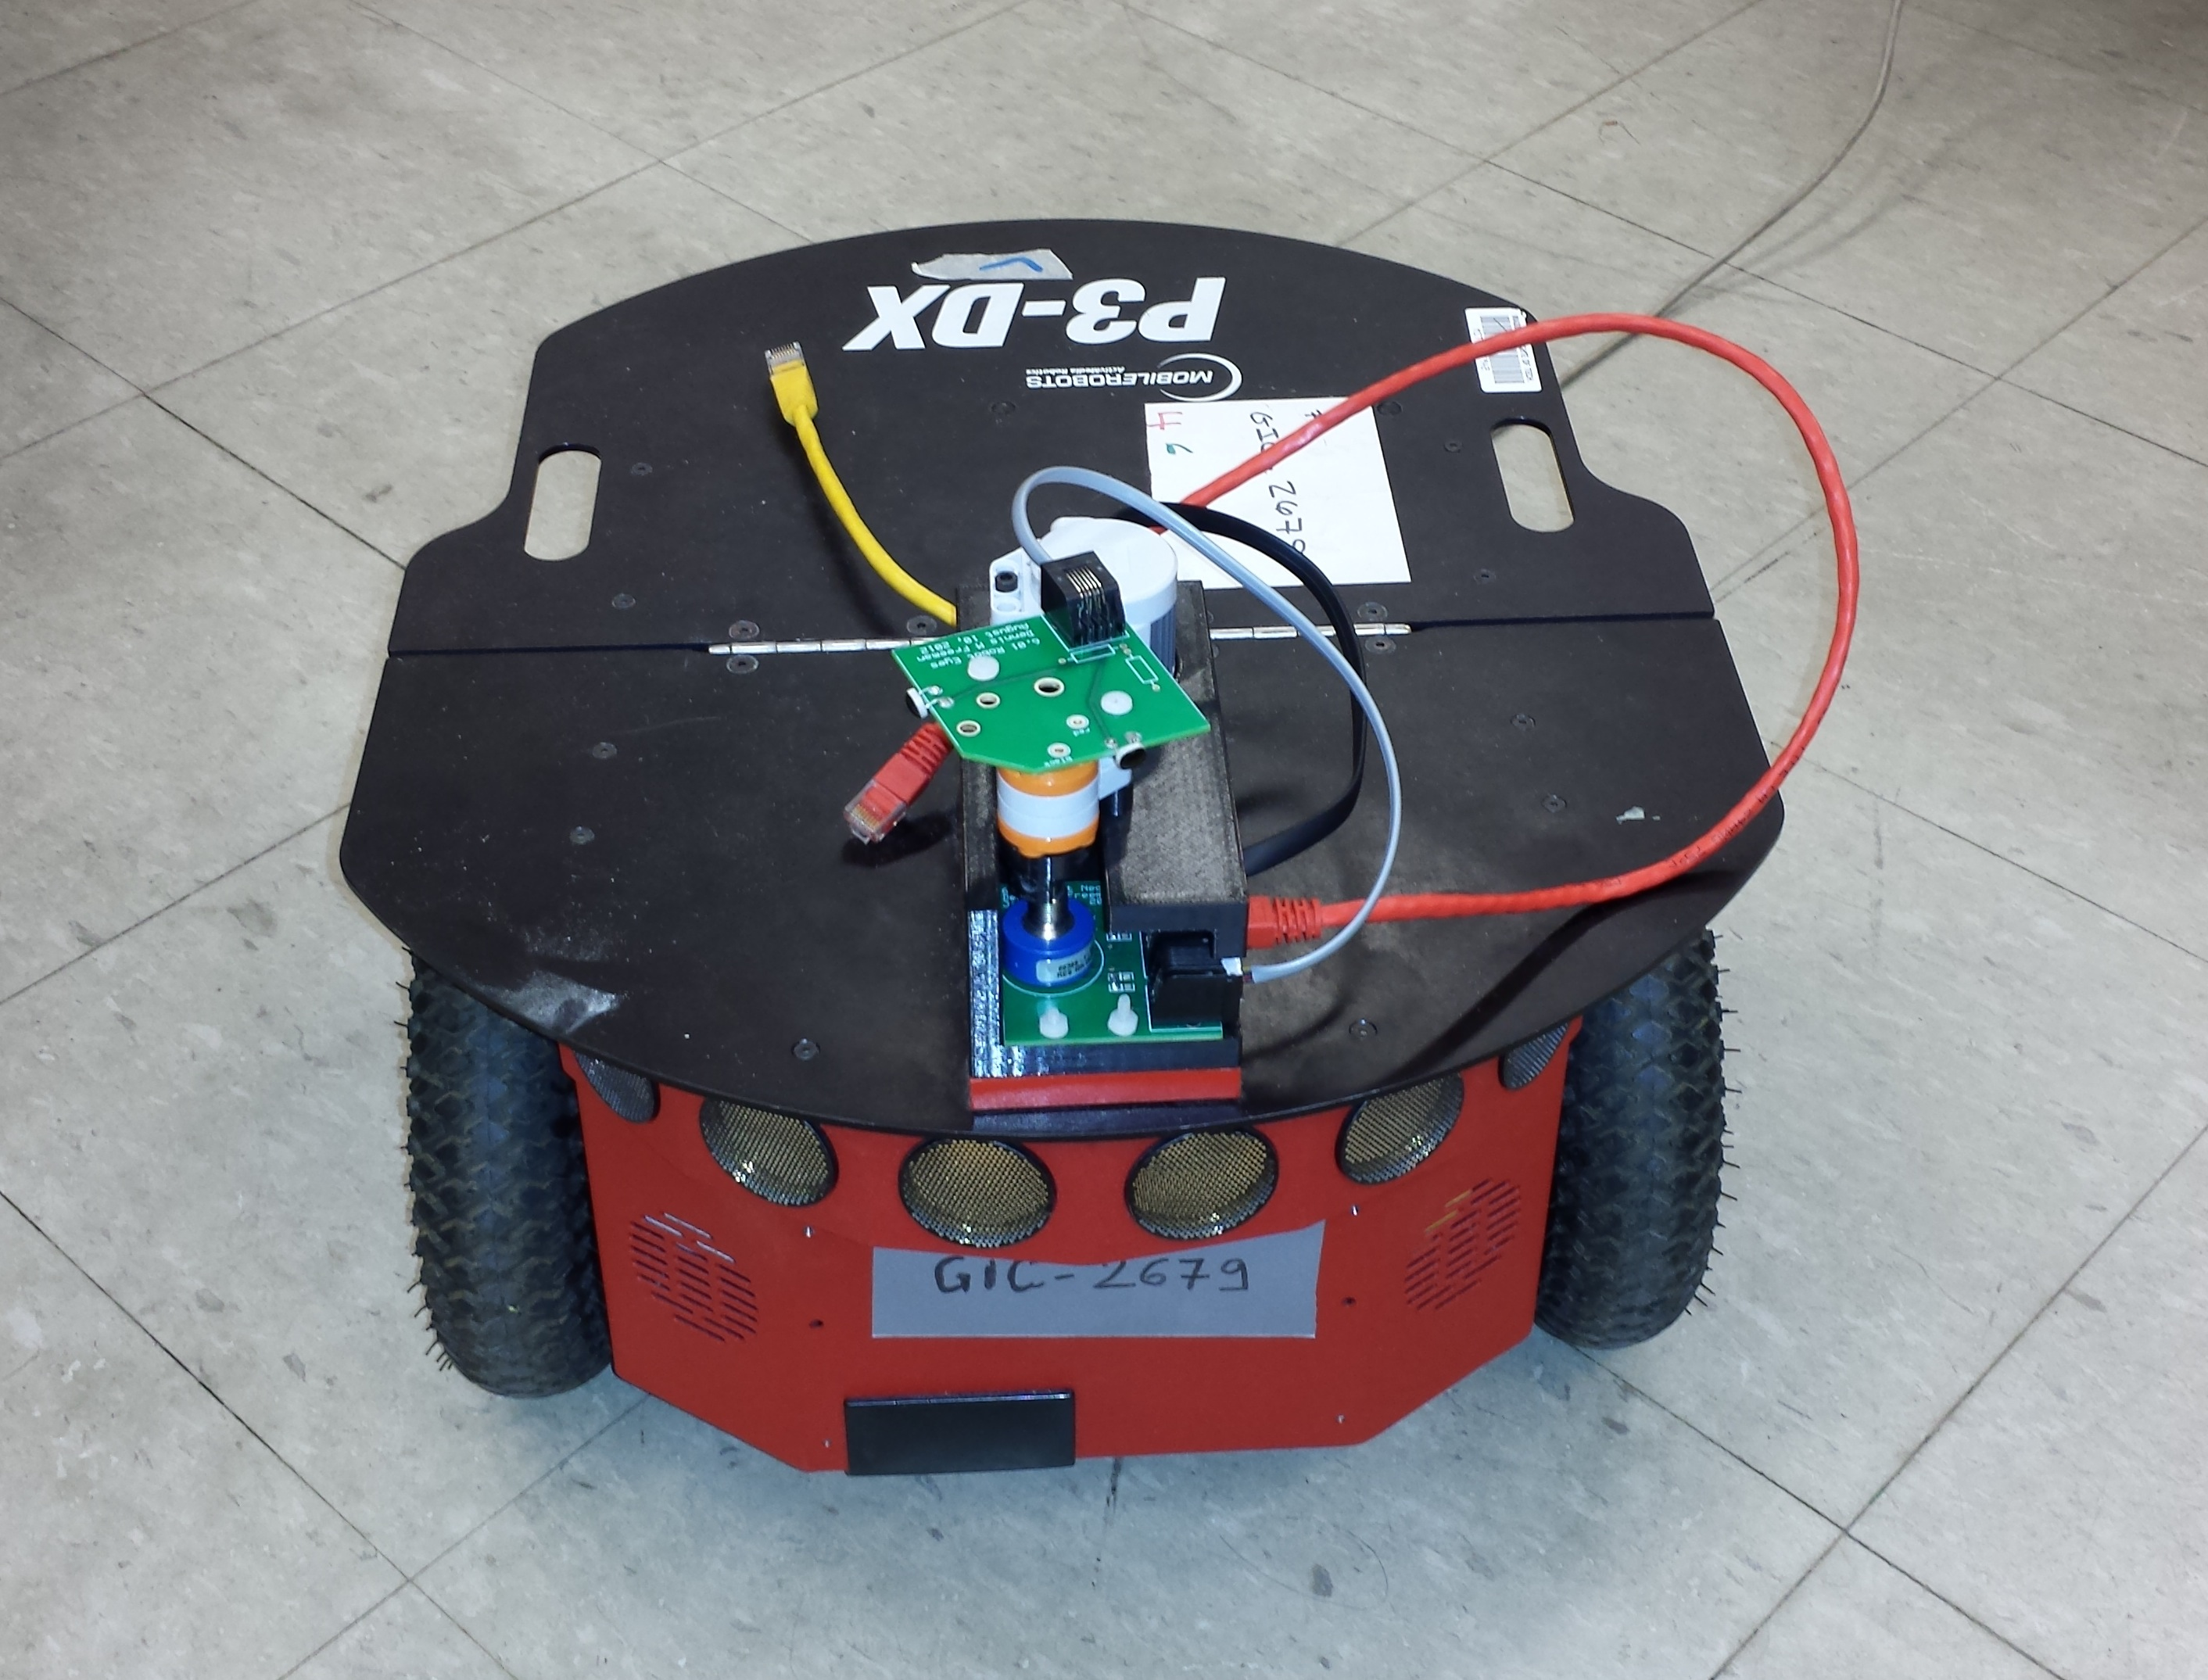
\includegraphics[width=\textwidth]{Images/robot.jpeg}
\caption[6.01 robot]{One of the 6.01 robots, with a head attached.}
\label{fig:robot}
\end{center}
\end{figure}

\begin{figure}
\begin{center}
\subfigure[Resistors]{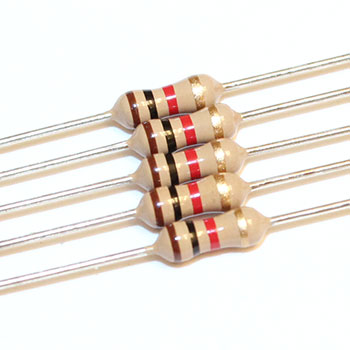
\includegraphics[width=5cm]{Images/resistors.jpg}}
\hspace{3cm}
\subfigure[Potentiometer]{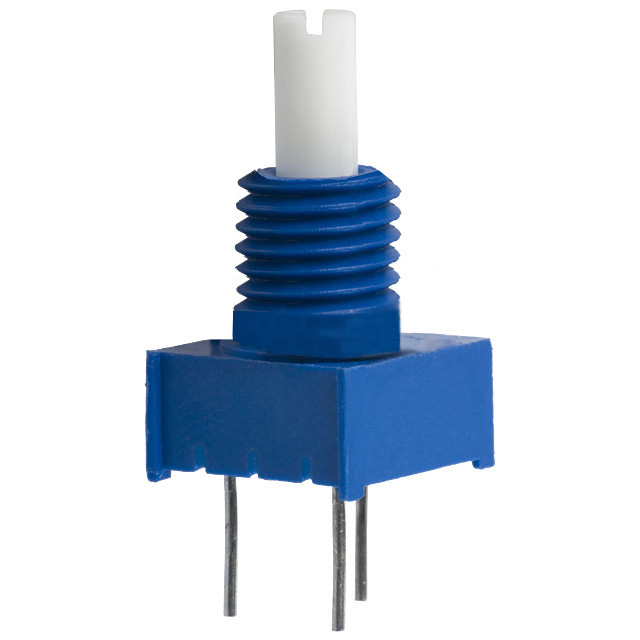
\includegraphics[width=5cm]{Images/pot.jpg}}\\
\subfigure[Operational Amplifier]{
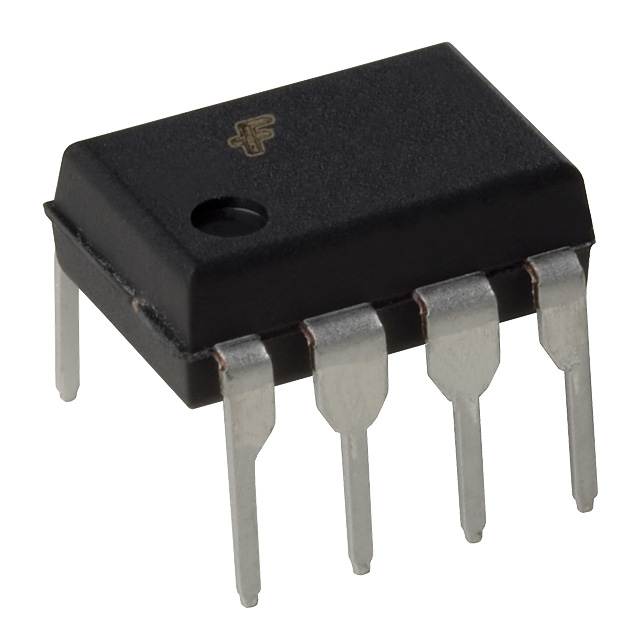
\includegraphics[width=5cm]{Images/op_amp.jpg}
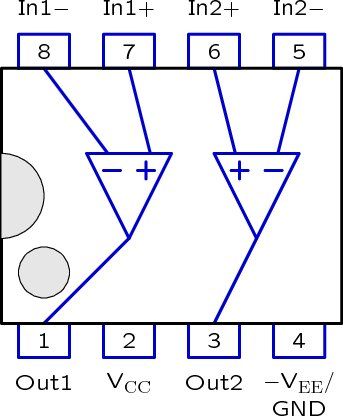
\includegraphics[width=4cm]{Images/op_amp_pin_out.jpg}
\label{fig:op_amp_pin_out}}\\
\subfigure[6-pin Motor Connector]{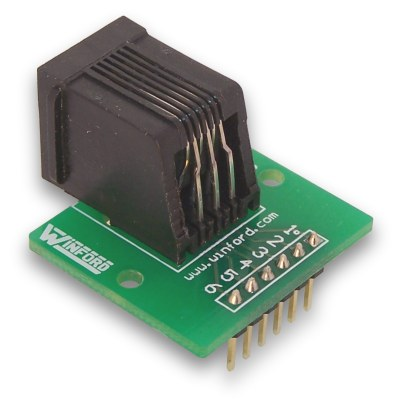
\includegraphics[width=5cm]{Images/6pin.jpg}}
\hspace{3cm}
\subfigure[8-pin Robot/Head Connector]{
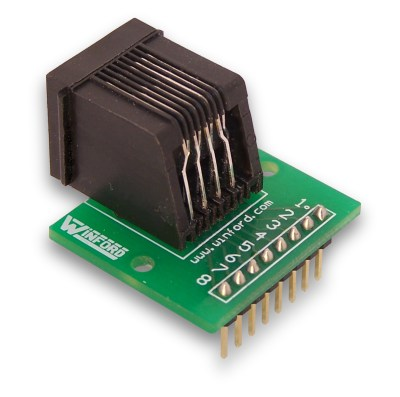
\includegraphics[width=5cm]{Images/8pin.jpg}}
\caption[Circuit pieces]{All circuit pieces used in 6.01 that may be
inserted into a protoboard.}
\label{fig:components}
\end{center}
\end{figure}

\subsection{Circuit Schematic}

Throughout this paper, the term \textit{circuit schematic} will refer to a
drawing, or a sketch, of a circuit containing its components and all the
interconnections between the components drawn as wires. This is what one would
sketch on a piece of paper in the process of designing a circuit. Figure
\ref{fig:schematic} presents an example of a circuit schematic.

\begin{figure}
\begin{center}
\includegraphics[width=\textwidth]{sample_schematic-22.mps}
\caption[Sample circuit schematic]{Sample schematic of a motor angular position
controller circuit.}
\label{fig:schematic}
\end{center}
\end{figure}

\subsection{Protoboard}
\label{sec:what_is_protoboard}

\textit{Protoboards} are boards on which one can quickly build and test
small circuits. They present a $2$-dimensional array of interconnected dots
in which circuit pieces and wires can be inserted. Figure
\ref{fig:physical_protoboard} presents an example of an empty
protoboard.
In the orientation depicted in Figure \ref{fig:physical_protoboard}, the first
two rows and the last two rows of dots (each pair having one row labeled with a
$+$ and the other row labeled with a $-$) are internally interconnected
horizontally. That
is, for each of these four rows, any two dots in the same row are connected
internally.
These rows are often referred to as the \emph{rails} and are often used for the
power and ground nodes, the $+$ rows being used for power, and the $-$ rows for
ground.
The group of rows labeled $A$ through $E$ in Figure \ref{fig:physical_protoboard}
can be better thought of as $63$ columns of 5 dots. Each of these groups of $5$
dots are connected internally. The same property holds for the columns within
rows $F$ through $J$. Henceforth, we will refer to an internally connected
group of $5$ dots on the protoboard as a $5$-column.

\begin{figure}
\begin{center}
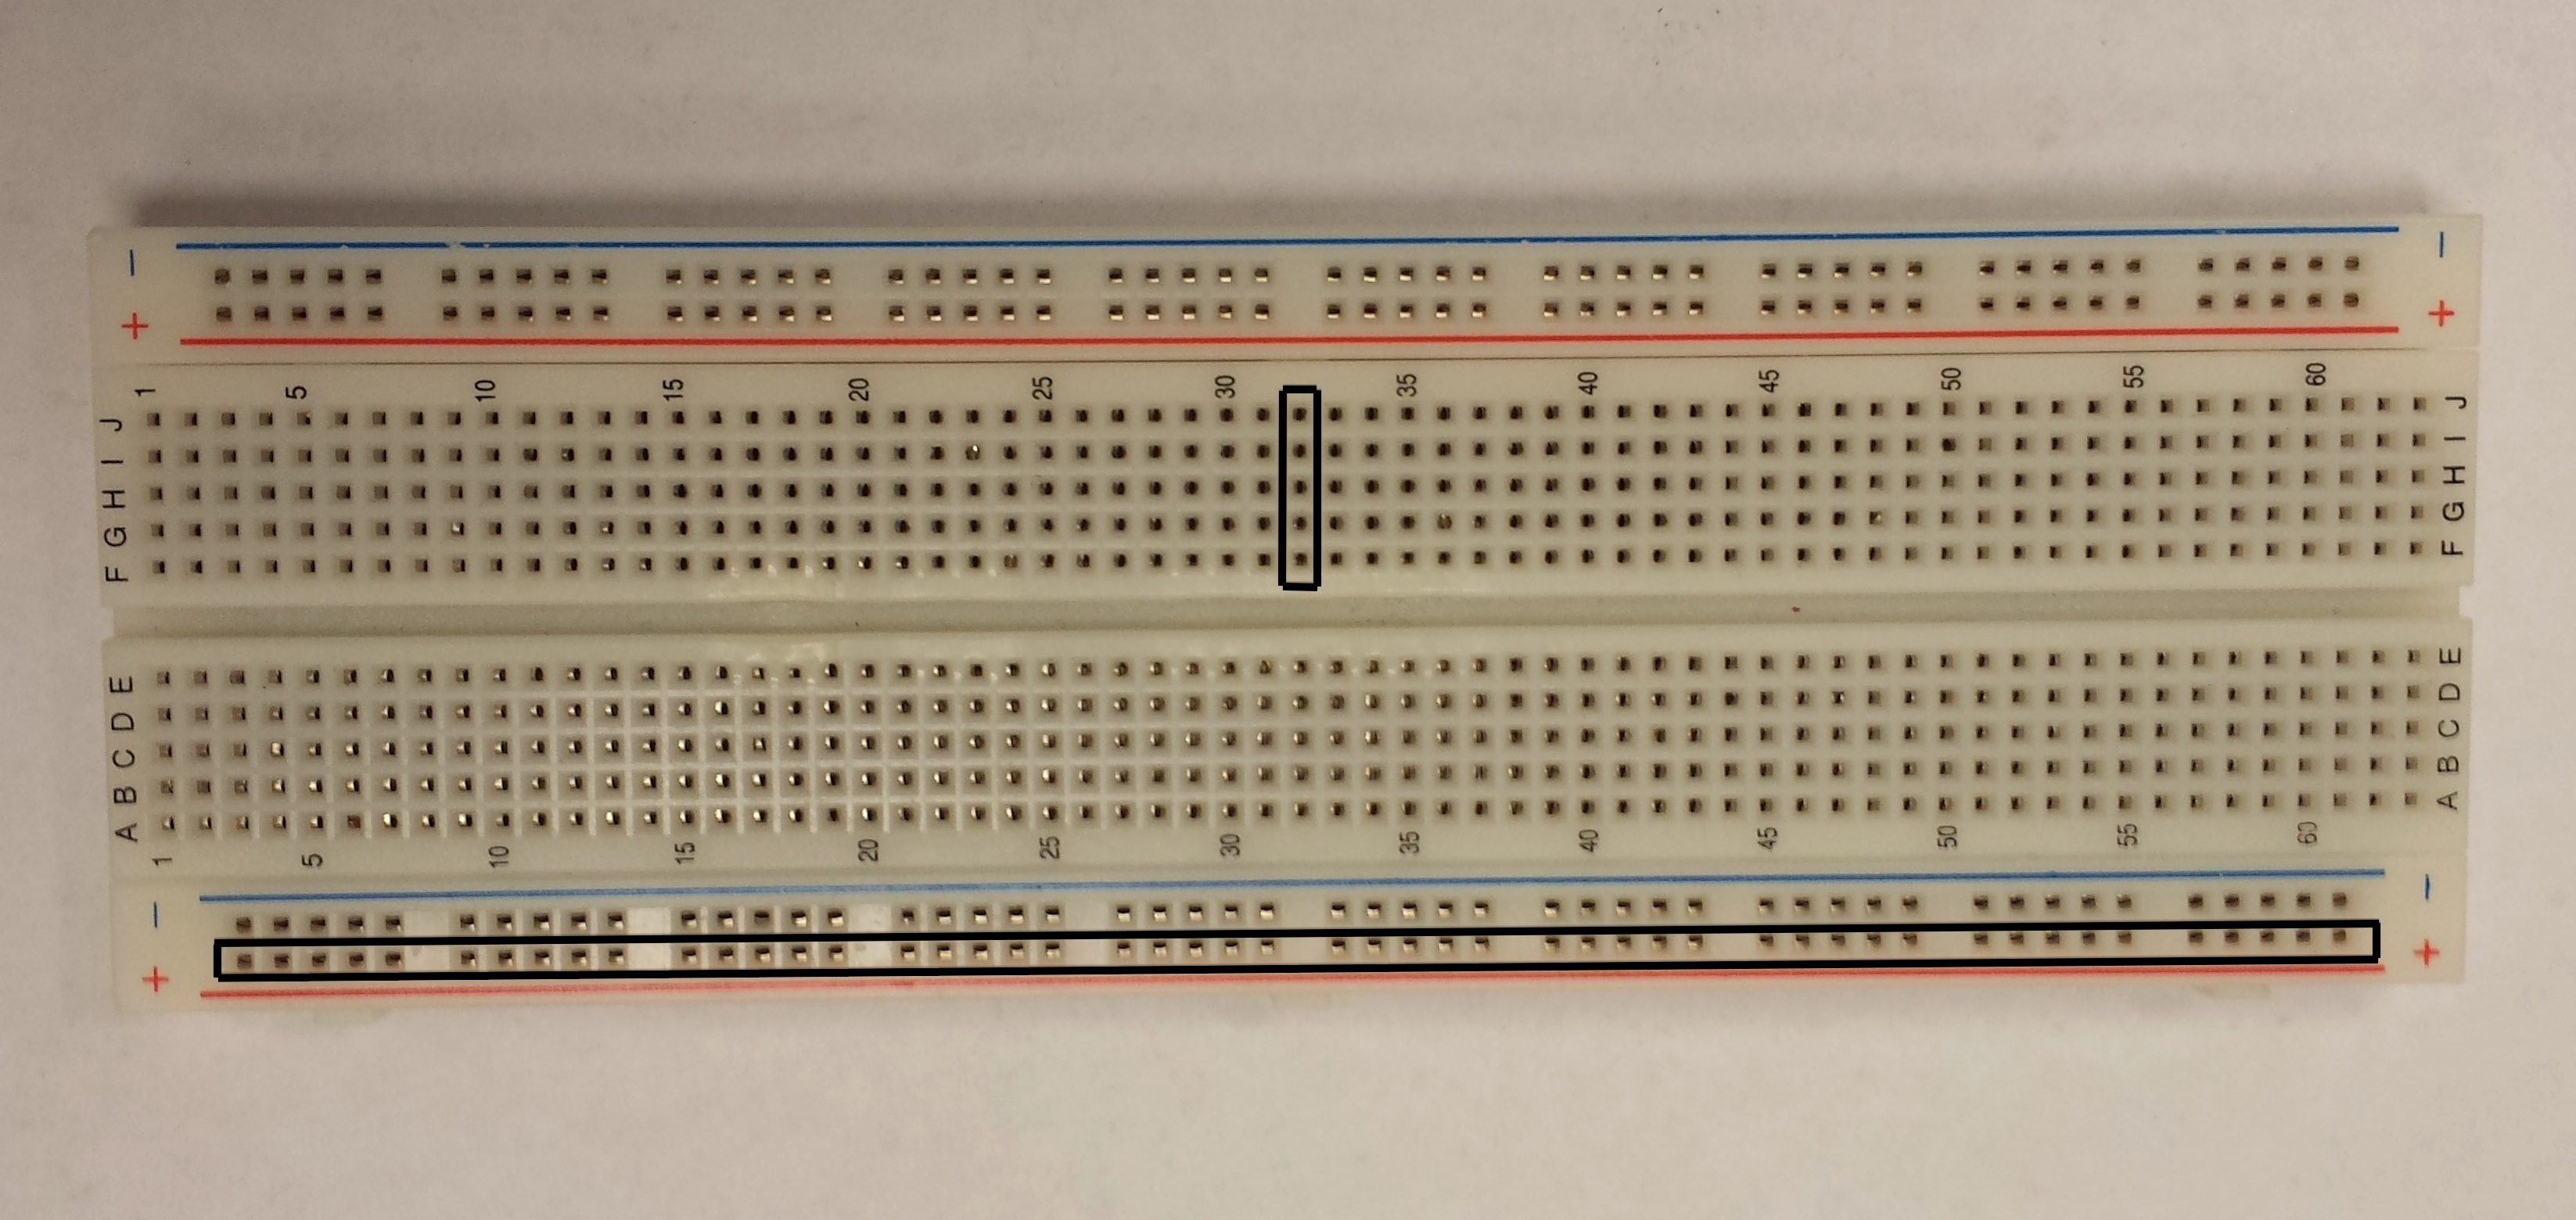
\includegraphics[width=\textwidth]{Images/physical_protoboard.jpg}
\caption[Protoboard]{A protoboard. In the rail rows, rows labeled with $+$ or
$-$, the dots are internally interconnected horizontally. In the middle two
groups of $5$-columns, the dots are interconnected vertically.}
\label{fig:physical_protoboard}
\end{center}
\end{figure}

\subsection{Protoboard Layout}
\label{sec:pb_layout}

A \textit{protoboard layout} of a given schematic is a placement of
circuit pieces
and wires on a protoboard that corresponds to the schematic. A protoboard layout
is constructed by
placing the appropriate pieces on the protoboard and then appropriately
interconnecting them with wires as prescribed by the schematic. As an example,
Figure \ref{fig:eg_s_to_pb} presents one possible protoboard layout
of the schematic shown in Figure \ref{fig:schematic}.

\begin{figure}
\begin{center}
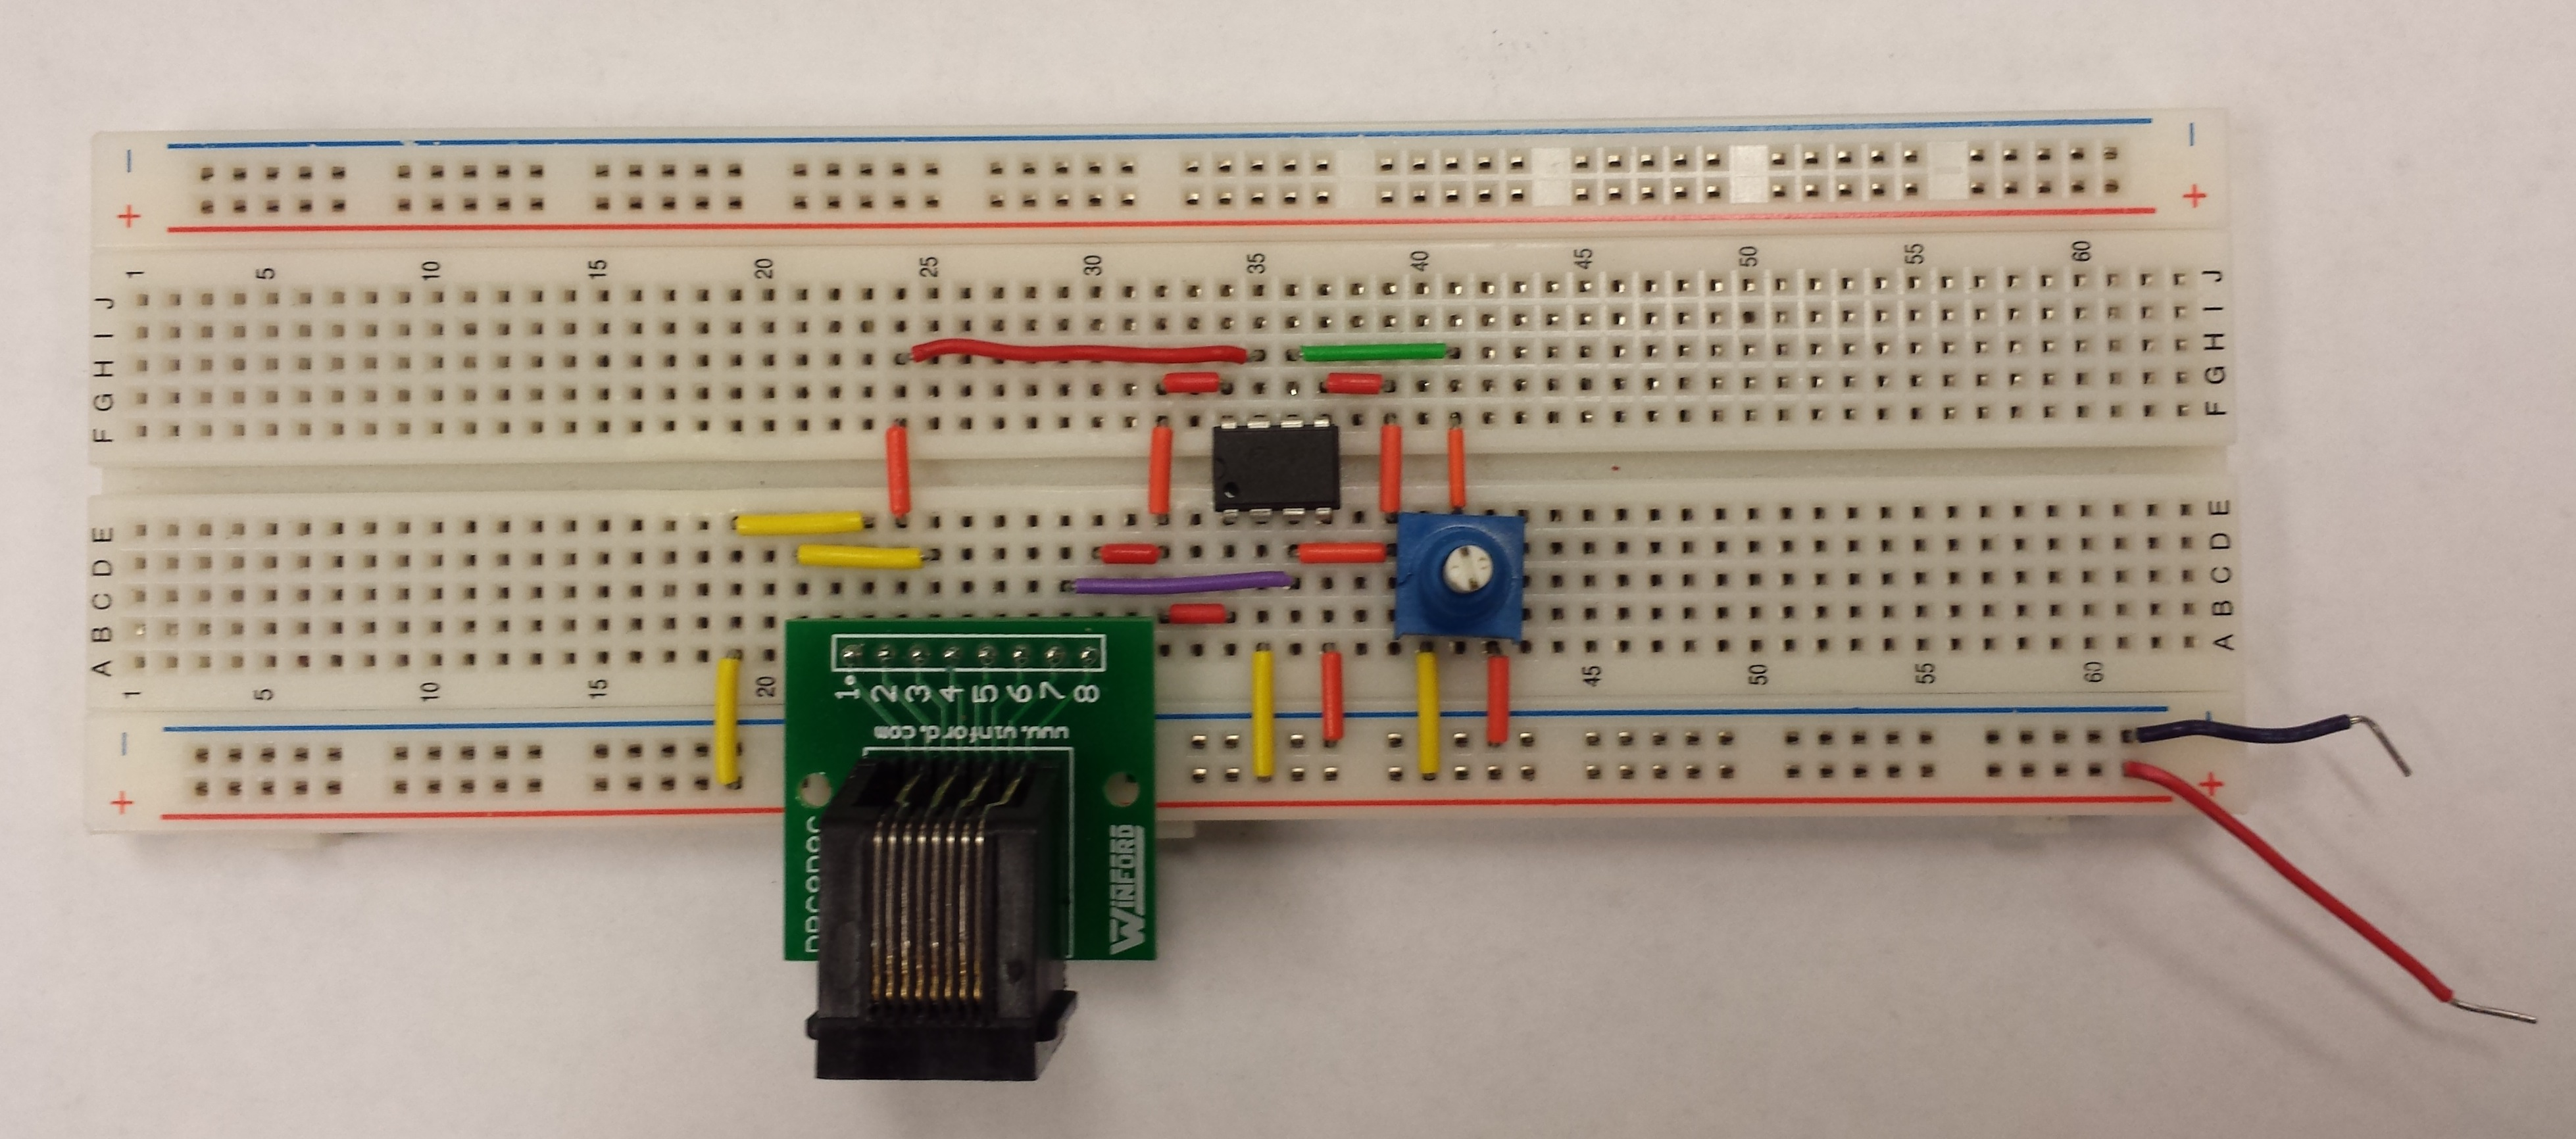
\includegraphics[width=\textwidth]{Images/sample_physical_layout.jpg}
\caption[Sample protoboard layout]{One possible protoboard layout of the
schematic shown in Figure \ref{fig:schematic}.}
\label{fig:eg_s_to_pb}
\end{center}
\end{figure}

For each of the circuit components we are interested in, there is a corresponding
circuit piece that may be inserted into the protoboard. The one exception is that
op-amps come in pairs. That is, as shown in Figure \ref{fig:op_amp_pin_out},
each op-amp circuit piece that is inserted in the
protoboard actually contains two op-amp components within it. This raises an
important design problem when laying out a schematic -- the need to find a
good way to group together the op-amps in a schematic to result in a ``good''
layout. To find the right packaging of op-amps and, furthermore, produce a
good layout all together, we need to first understand what makes a layout good.
There are no conclusive ways to tell whether a layout is good, but, keeping in
mind that we want layouts that are easy to build,
easy to debug, and aesthetically pleasing, we could come up with the
following rules of thumb:
\begin{itemize}
\item The layout should not have any wires that cross circuit pieces.
\item The layout should have no crossing wires, especially occlusions (i.e.,
crossing wires with the same orientation).
\item The layout should consist of only horizontal and vertical wires (i.e., no
diagonal wires).
\item The layout should have as few wires as possible.
\item The total length of wires in the layout should be as small as possible.
\end{itemize}

Given the background information discussed thus far, the goal of this project is
automatically generating a ``good'' protoboard layout from a circuit schematic.

\section{Previous Work}

Here we discuss previous work that has been done relating to this project.
First, as our project aims to augment the quality of 6.01, we look at the
infrastructure currently used in 6.01. Next, we look at what work has
been done relating to layout in general.

\subsection{CMax}

In a typical circuits lab in 6.01, students first design their circuits by
drawing schematics of the circuits on paper.
After iteratively improving their designs based on discussions with staff
members, they lay out their circuits on a simulation tool called Circuits Maximus
(CMax)\cite{cmax}. Note, therefore, that students currently lay out their
circuits themselves.
With CMax, a student can lay out a circuit on a simulated protoboard, and test
the circuit to make sure that it behaves as desired. CMax provides a fast
and safe way of debugging circuit layouts compared to debugging layouts on a
physical protoboard. Once the students are satisfied with their
observations from CMax, they build their circuits on physical protoboards and
carry out the appropriate experiments. Figure \ref{fig:cmax_sample} presents one
possible protoboard layout, as depicted in CMax, of the schematic shown in
Figure \ref{fig:schematic}.

\begin{figure}
\begin{center}
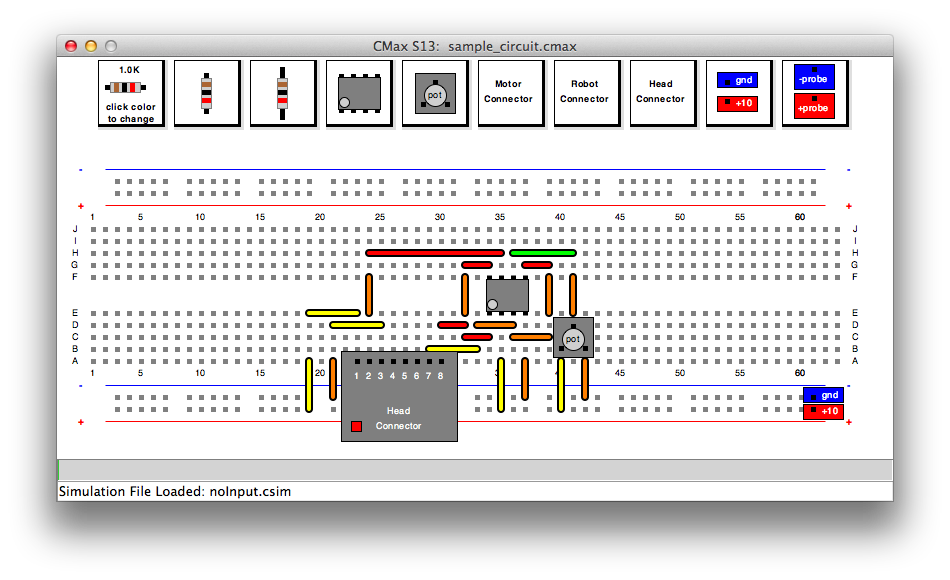
\includegraphics[width=\textwidth]{Images/sample_circuit.png}
\caption[CMax]{One possible CMax layout for the schematic shown in Figure
\ref{fig:schematic}.}
\label{fig:cmax_sample}
\end{center}
\end{figure}

Using CMax has reduced circuit debugging time for 6.01 students.
Its introduction has made
learning circuits significantly easier for many students, especially those that
have little or no prior experience with circuits. In addition to making the lab
exercises more manageable, it provides students with a way to
build, analyze, and experiment with circuits at their own leisure outside of lab.

A potential weakness of circuits labs in 6.01 as they are currently given is
that student have to produces the protoboard layouts themselves.
While generating protoboard layouts
of circuit schematics may have instructive substance, a student's time is better
spent thinking about designing circuits in the first place.
Currently students design circuits by drawing schematic diagrams on paper.
Once they are happy with
their schematic diagrams, they proceed to laying out the corresponding circuits
with CMax. When the circuits get complicated and involve many pieces,
translating a
schematic diagram into a protoboard layout becomes quite challenging and
time-consuming. In these situations, students often end up with convoluted
layouts that are difficult to debug in the case of the
circuit not behaving as expected. Not only are such layouts difficult for the
students to debug, but they are also often difficult for staff
members to understand. In the best case scenario, students should have to work
out the right schematic diagram for the circuit they are designing,
but should not have
to produce the corresponding protoboard layouts.

With the schematic entry tool this paper introduces, a typical 6.01 circuits lab
would proceed as follows. First, as before, students would draw schematic
diagrams of their circuits on paper. Once they have
schematic drawings they are happy with, they would recreate their schematic
drawings on the schematic entry tool. In fact, students may proceed directly to
building the schematic drawings on the tool, bypassing the
experimentation on
paper. Once they have a schematic drawn, they would analyze it with the tool,
discuss it with staff members, and improve it with the tool. When they are
satisfied with the behaviors of their schematic circuit, they would produce the
corresponding protoboard layout automatically. The automatic generation of
protoboard layouts would be
the most important advantage of this tool. They would then build the layout on a
physical protoboard and carry out experiments with it.

\subsection{Current Work in Automatic Layout}
\label{sec:prev_layout}

In my explorations, I was not able to find any tools that
automatically translate circuit schematics into protoboard layouts.
However, there
do exists tools, such as Cadence\cite{cadence} and EAGLE\cite{eagle},
that perform partially- or fully-automatic Printed Circuit
Board layout. To my findings, the owners of these tools have not published
their algorithms. Hence, I was not able to build my
work off of any existing products. In a sense, this project aims to build
something new.
